\documentclass[11pt,a4paper]{article}

\usepackage{amsmath} %for mathemathic formulas
\usepackage{amssymb}
\usepackage[ngerman]{babel} %for the german language by the spellling reform (without the package the date would look like April 20, 2020)
\usepackage{enumitem} %for enumeration surrounding 
\usepackage{graphicx} %for pictures
\usepackage{siunitx}

\title{Blatt 2}
\date{\today}
\author{Hannah Rotgeri \and Feline Heinzelmann}

\begin{document}
    \maketitle

    \section*{Aufgabe 1}
    	\begin{enumerate}
		\item[a)] Die Brillanz ist einserseits proportional zur Photonenzahl, andererseits umgekehrt proportional zu Zeit, zur Fläche, zum Raumwinkel und zum Wellenlängenbereich. Sowohl der Wellenlängenbereich als auch die Winkeldivergenz ist bei bei einer Röntgenröhre deutlich größer als bei einer Synchrotronstrahlungsquelle. In einer Synchrotronstrahlungsquelle werden die Elektronen relativistisch beschleunigt, was zu einem starken Energieverlust der beschleunigten Teilchen führt. Außerdem sorgen die eingesetzten Undulatoren für ein extrem schmalbandiges Spektrum. Des Weiteren wird die Strahlung innerhalb solcher Beschleunigungsstrukturen gepulst abgeben \( B \propto 1/t \). \\
		
		In einer Röntgenröhre können leichter hohe Energien erreicht werden, da die Elektronen ihre kinetische Energie vollständig umwandeln, wenn sie auf die äAtome der Anode treffen. (Jedoch ist der Wrkungsgrad \( \eta < 1\% \) aufgrund von Wärmefreigabe). Im Gegensatz verlieren die Elektronen in einer Synchrotronstrahlungsquelle nur einen Teil ihrer Energie in Form von Synchrotronstrahlung. Ein weiterer Aspekt ist folgender: Die Energie in Röntgenröhrern ist leichter durch die starke Abhängigkeit von der Beschleunigungsspannung zu variieren. Bei Synchrotronstrahlungsquellen ist der Energieverlust und damit die Energie des entstehenden Photonenstrahl im Wesentlichen vom Radius des Speicherrings abhängig, sodass der Aufwand zur Änderung größer wäre.
		\item[b)] Nicht nur die Energie der Teilchenstrahlung ist zur Erzeugung von effizienter Synchrotronstrahlung entscheidend, sondern auch die Intensität der Photonenstrahlung. In heutigen Synchrotronstrahlungsquellen sind Undulatoren verbaut, mit denen es gelingt, die abgegebene Photonenstrahlung der im Magnetparcours durchlaufenen relativistischen Elektronen in einer Richtung zu überlagern \(I = \frac{\Delta E}{\Delta t * A}\)
	\end{enumerate}
	
    \section*{Aufgabe 2}
	
	\begin{enumerate}
   		\item[a)] Wellenlänge der Synchrotronstrahlung: $$ \omega_\text{typ}=\frac{3\pi c \gamma^3}{2 \rho}$$.
        	Dabei ist $\gamma=30\,$MeV$/511\,$keV und der Radius und $\rho= 0.293\,$ m. 
        	Damit ergibt sich eine Wellenlänge von 307$\,$nm, was nicht im sichtbaren Bereich liegt.
    		\item[b)] Strahlungsverlusst: $P_s=\frac{e²c}{6 \pi \epsolon_0 (m_ec²)⁴} \cdot \frac{E⁴}{R²} = \SI{8.887}{\joule			\per\second}$ \\
		mit $R$ als Biegeradius und $E$ als Strahlendergie. \\
		Uns ist nicht ganz klar, ob der Hinweis in der Aufgabe bedeutet, dass alle emittierten Photonen auf der Diode ankommen 			oder durch den Abstand zum Strahl nicht. Wäre die Diode nicht in der Vakuumkammer, würde der Photonenstrahl duch die 			Kammerwand und die Luft zwischen Kammer und Diode abgeschwächt und gestreut.
    		\item[c)] Anzahl Elektronen: $N= Q/e = I \cdot R/c = \num{2.3e11}$.
                Verhältnisse mit und ohne kohärente Strahlung: $\frac{N + (0.001 \cdot N )^2}{N} = 1 + \num{e-6} \cdot N = \num{2.3e5} $
	\end{enumerate}

    \section*{Aufgabe 3}
        Elektron: \\
            Kreisumfang \(U = \SI{100}{\metre}\)
            Geschwindigkeit = \( v = 0.99*c \)
        \begin{figure}[h]
            \centering
            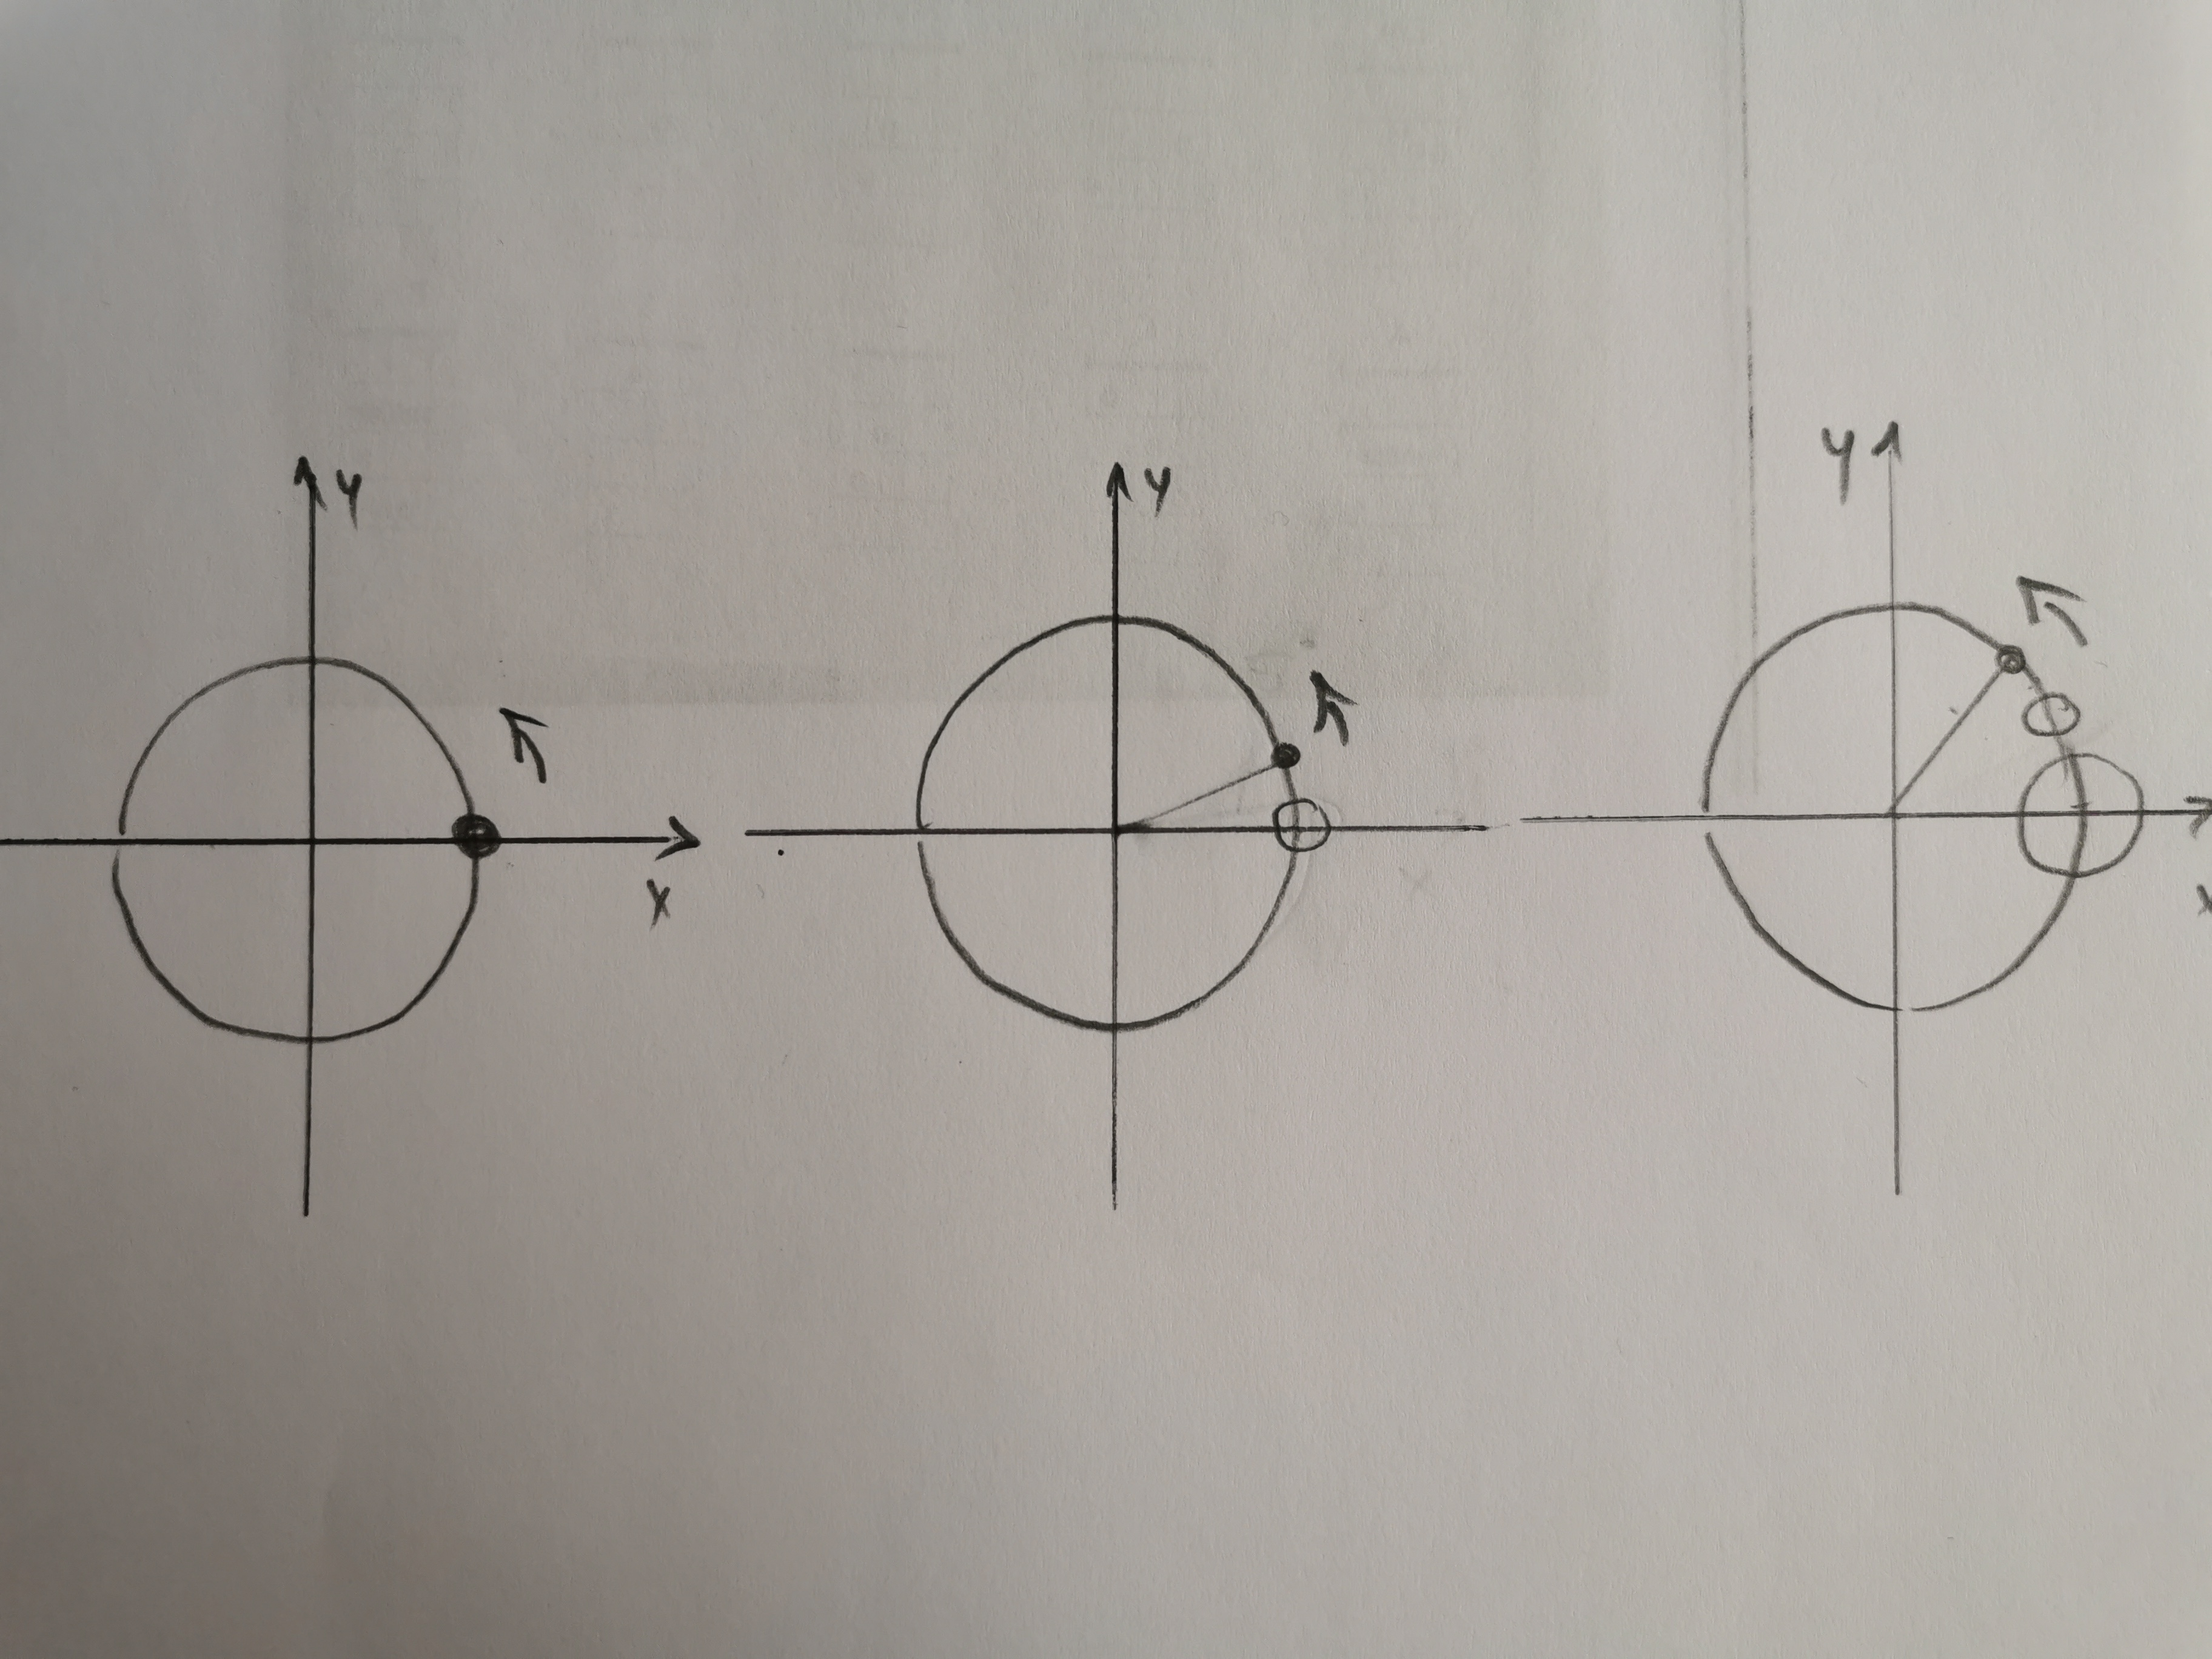
\includegraphics[width=0.7\textwidth]{Synchrotron_Skizze.jpg}
            \caption{Skizze mit der Bewegung eines Elektrons und seiner abgestrahlten Synchrotronstrahlung entlang seiner Kreisbahn}
        \end{figure}
        \begin{enumerate}
            \item Schritt: Zeit für einen Durchlauf berechnen \( t_{\mathrm{D}} = \frac{u}{v} \approx \SI{337}{\nano\second}\) 
            \item Schritt: Zeit für zwei Durchläufe berechnen, da Simulation der Synchronatronstrahlung nach zwei Runden gefragt ist \\
            \( t_{\mathrm{Stop}} = 2*t_{\mathrm{D}} \approx \SI{675}{\nano\second}\) 
            \item Schritt: Bewegung des Elektrons simulieren (Kreis)
            \item Schritt: Elektron auf Kreisbahn zu jeder Position auf dem Kreis zeichnen anhand trigonometrischer Beziehungen \\
            (\( x = r * \cos(\omega * t_{ \mathrm{aktuell} } ) , \, y = r * \sin(\omega * t_{ \mathrm{aktuell} } ) \))
            \item Schritt: Radius der Synchrotronstrahlung bestimmen \\
            \( r_{\mathrm{Syn}} = c*(t_{ \mathrm{aktuell} } - i * t_{ \mathrm{Strahlungserzeugung} } ) \) , 
            wobei i der i-te Strahlungskegel ist, der in jeweils \( 5 ^\circ\) Abständen durch das Elektron erzeugt wird; \\
            mit \( t_{\mathrm{Strahlungserzeugung}} = \frac{t_{\mathrm{D}}}{72} \) mit \( \frac{360 ^\circ}{5 ^\circ} \) 
            (Radius entspricht der Entfernung, die das Licht seit der Emission zurücklegt)
            \item Schritt: Synchrotronstrahlungskreise für zwei Umläufe zeichnen mit jeweiliger Position der Synchrotronkreise 
            nach jeweils \( 5 ^\circ\) und mit jeweiligem Radius zur betrachteten aktuellen Zeit 
        \end{enumerate}

        \begin{figure}[h]
            \centering
            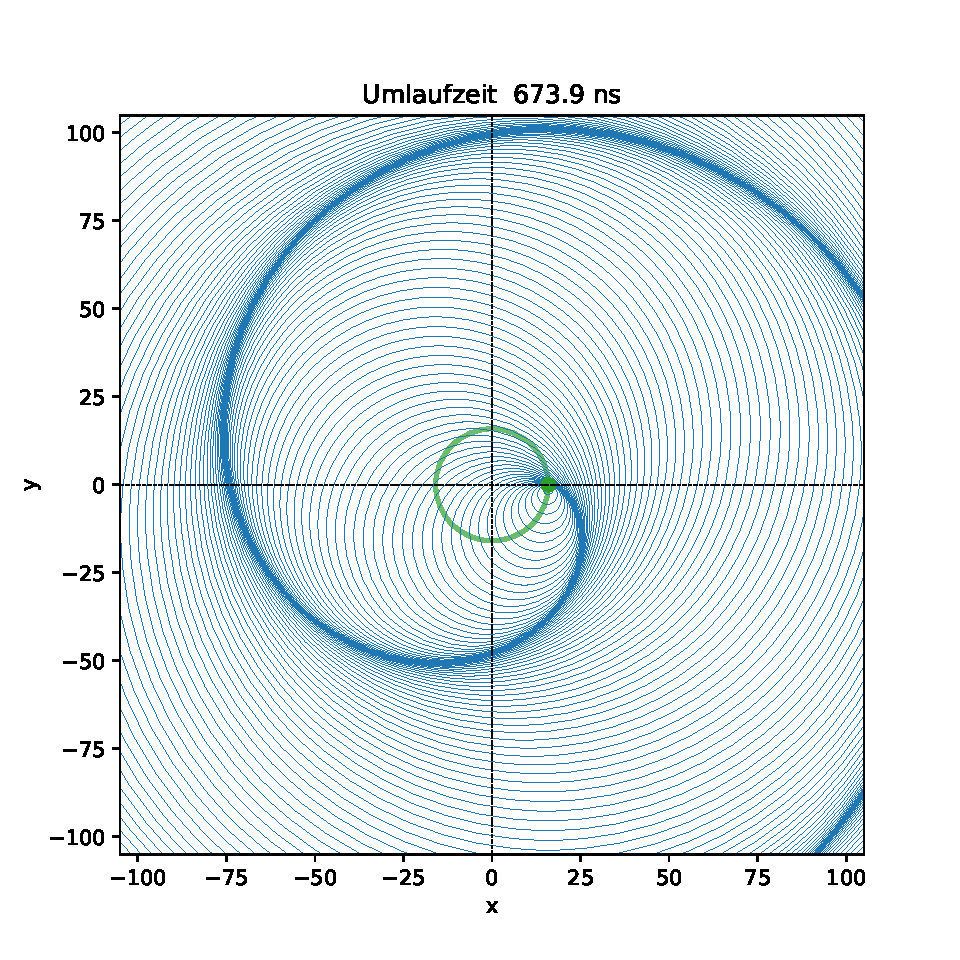
\includegraphics[width=0.7\textwidth]{synchrotron-0673.9.pdf}
            \caption{Emission von Synchrotronstrahlung nach zwei Umläufen}
        \end{figure}

        \begin{figure}[h]
            \centering
            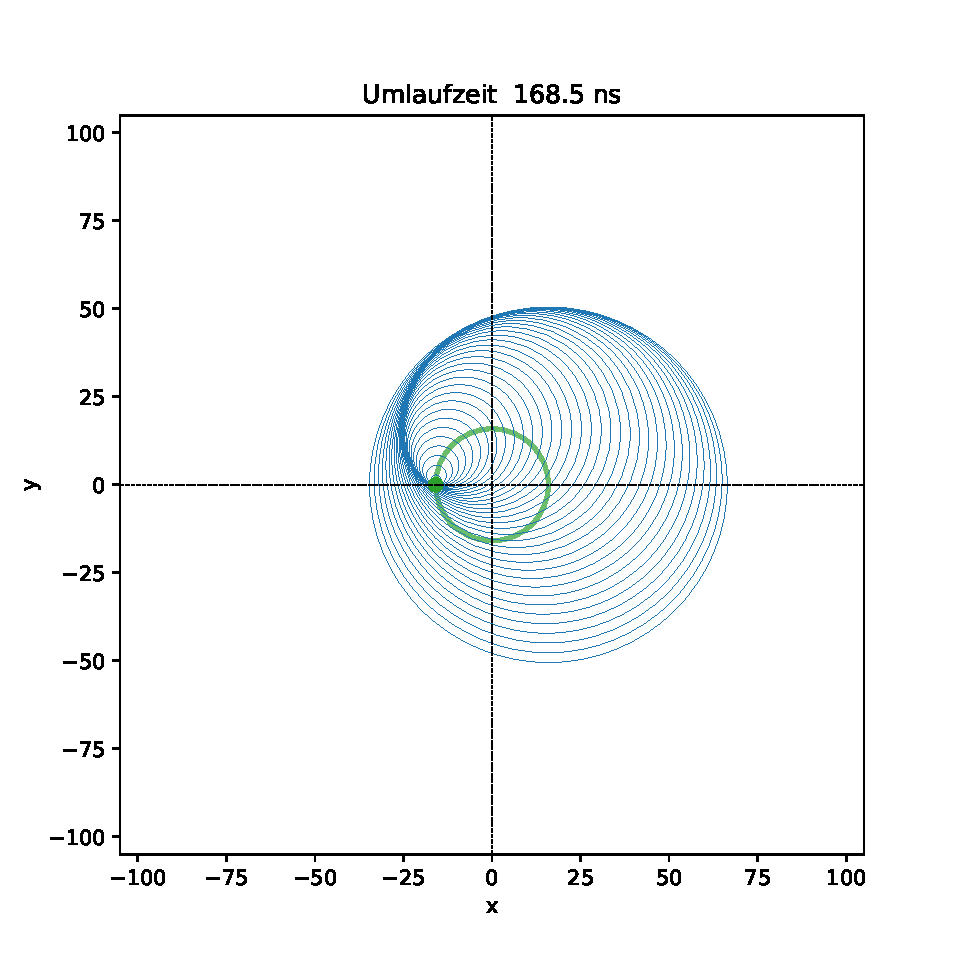
\includegraphics[width=0.7\textwidth]{synchrotron-0168.5.pdf}
        \end{figure}

        \begin{figure}[h]
            \centering
            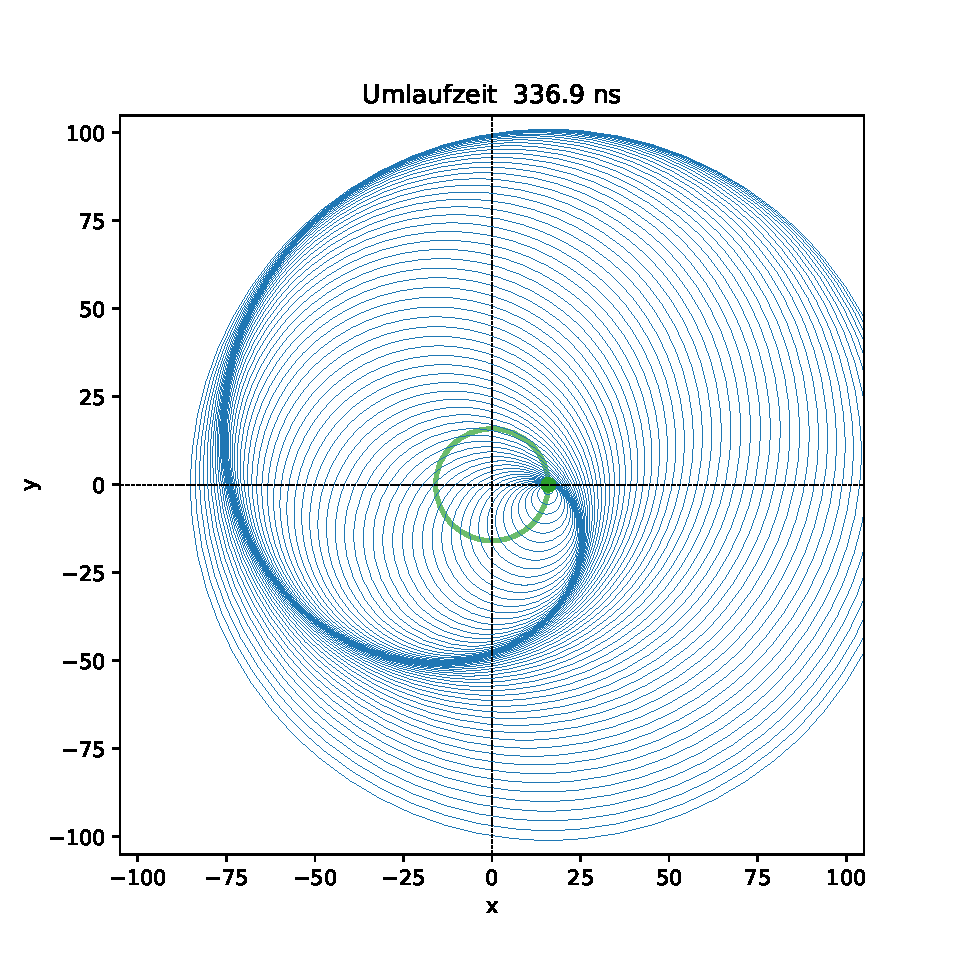
\includegraphics[width=0.7\textwidth]{synchrotron-0336.9.pdf}
        \end{figure}

\end{document}


